\chapter{研究背景}
\label{chap:background}

本章では既存のARナビゲーションシステムの現状と、その問題点を整理する。

\newpage


\section{ARによるヘルプ・ナビゲーションシステム}
ARによる表示をヘルプやナビゲーションシステムに利用する研究はは90年代はじめから存在する。
初期の有名な例としてはプリンタのメンテナンス情報をARで表示するプロトタイプである、KARMA\cite{10.1145/159544.159587}や大学構内の案内をARで表示するナビゲーションシステムであるA Touring Machine\cite{629922}が挙げられる。
これらはヘッドマウントディスプレイを利用したものであるが当時のヘッドマウントディスプレイは非常に大型で性能の限界もあり実用的とは言えないものであった。

その後2000年代になりモバイル端末が普及するとGPSと方位などの情報をもとにカメラを通して周囲の情報をディスプレイに表示するアプリケーションが現れるようになった。
代表的なものとしてWikitude\footnote{\textsf{https://www.wikitude.com/}}が挙げられる。


\section{ARによるヘルプ・ナビゲーションの現状}
\label{current}
ARによるヘルプ・ナビゲーションとして実用化しているシステムを紹介し、その現状を解説する。

\subsection{Google MapsのARナビ機能}
Google \footnote{\textsf{https://google.com}}は2018年のGoogleI/O 2018で自社の開発する地図アプリケーションGoogle Maps\footnote{\textsf{https://www.google.com/maps}} にAR機能が追加されることを発表し、翌2019年5月にARナビゲーション機能としてα版をリリースした。
この機能ではGPSによる位置情報や方位情報、カメラからの画像情報などをもとに図\ref{fig:googleMapAr}のようなAR表示での道案内を表示する事が可能である。
本アプリケーションはカメラで取得した周囲の景色による補正からかなり高精度なAR表示を提供するが、用途はあくまでもあくまでも目的地までの経路案内に限られている。
またGPSの届かいない場所やGoogleStreetViewなどに景色の登録がない施設では利用ができないと言うデメリットが存在している。

\begin{figure}[h]
  \begin{center}
      \includegraphics[width=60mm]{images/google-maps-ar-mode.png}
  \end{center}
  \caption{Google MapsでのAR表示} \label{fig:googleMapAr}
\end{figure}

\subsection{遺跡・史跡のARナビゲーションアプリ}
また日本国内の史跡ではマーカーベースのAR案内アプリケーションが複数存在しているしている。
殆どのものが史跡の近くにマーカーを設置し、そこから解説や当時の様子を再現したCGを描くというものである。
今回は一例として松山城址でのナビゲーションアプリである「攻略 松山城」\footnote{\textsf{https://www.cadcenter.co.jp/works/archives/98}}を紹介する。
このアプリは松山城の歴史や仕組みを解説するARナビゲーションアプリである。
図\ref{fig:matsuyama_marker}の専用のマーカーをアプリのカメラで読み込むことで図\ref{fig:matsuyama_ar}のように解説動画のリンクをを適切な位置に表示する。
このようなアプリの場合、表示したい場所ごとに図\ref{fig:matsuyama_marker}のような大きなマーカーを設置しなければならないと言う問題点がある。
また実際の運用を考えると専用のマーカーとアプリを利用しているため、多くのマーカー付近でアプリをダウンロードするための案内が別途必要になり、汎用性があるとは言い難い。


\begin{figure}[h]
  \begin{minipage}{0.5\hsize}
    \centering
    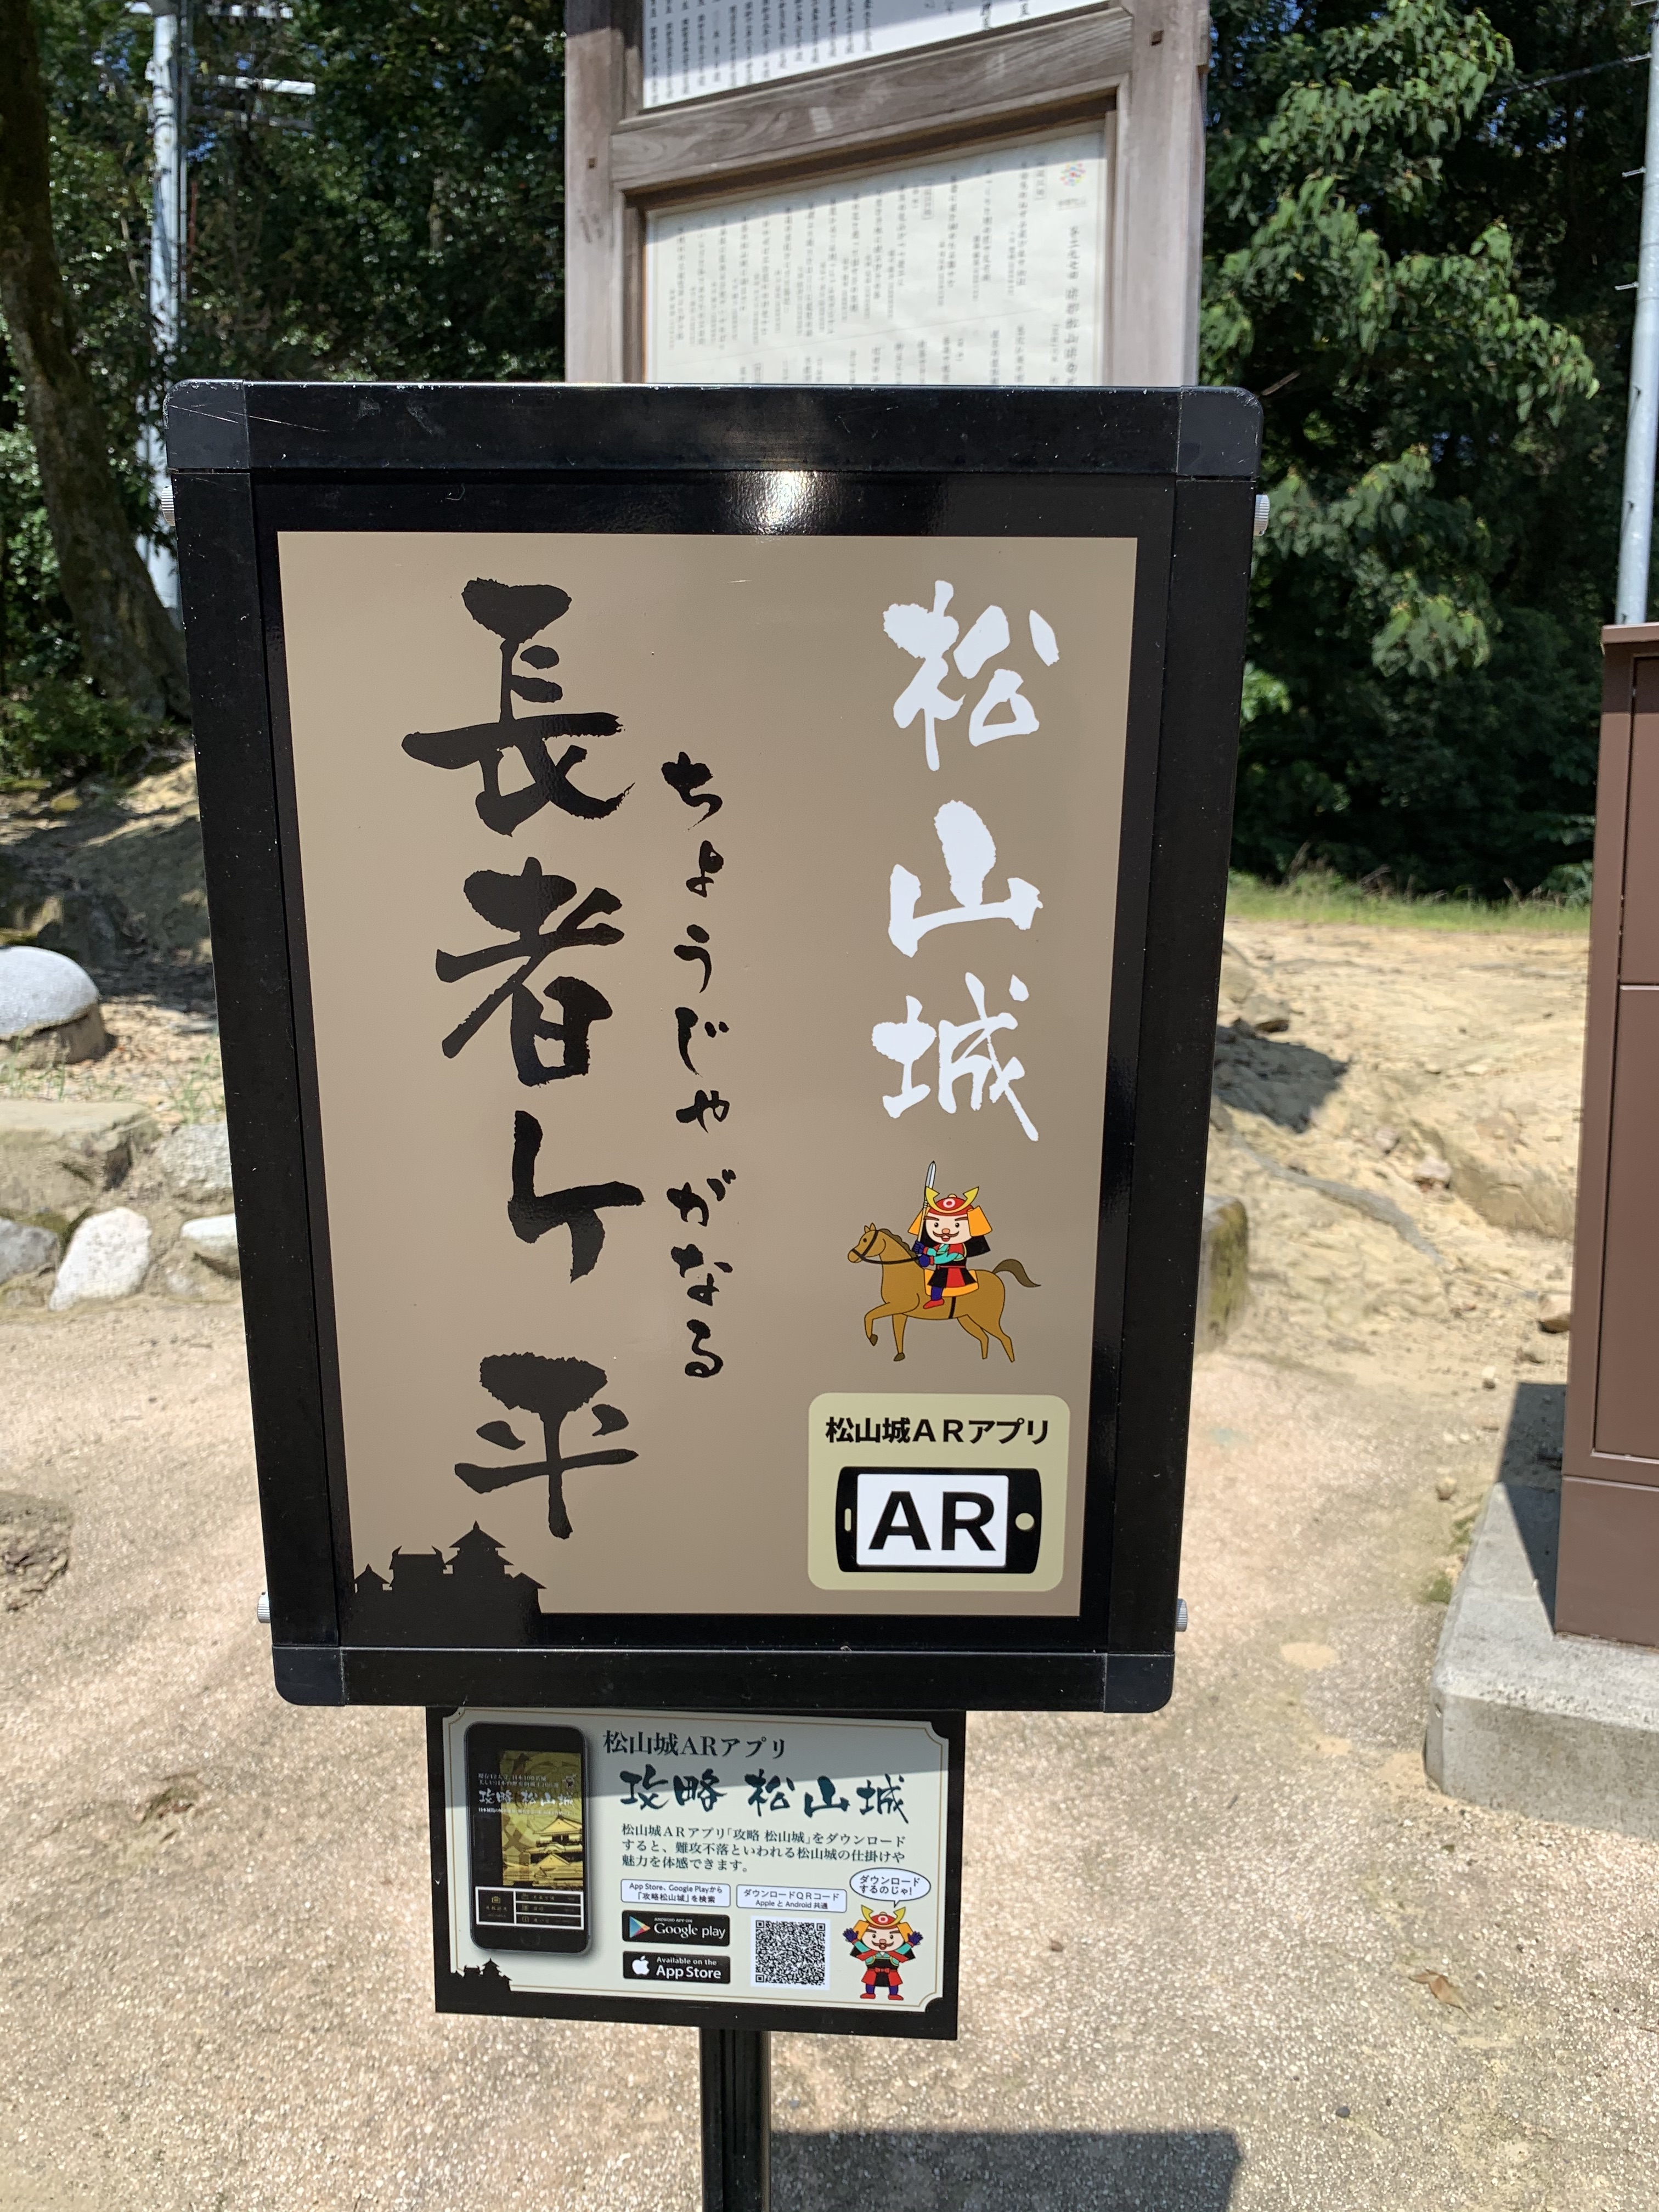
\includegraphics[width=70mm]{images/matsuyama_marker.jpg}
    \caption{専用のマーカー} \label{fig:matsuyama_marker}
  \end{minipage}
  \begin{minipage}{0.5\hsize}
    \centering
    \includegraphics[width=60mm]{images/matsuyama_ar.png}
    \caption{ARでの案内} \label{fig:matsuyama_ar}
  \end{minipage}
\end{figure}


\section{ARによるヘルプ・ナビゲーションの問題点}
\label{problems}
前節で述べた現状を元に既存のARによるヘルプ・ナビゲーションシステムの問題点を整理する。
ARのナビゲーションシステムには以下のような問題点がある。

\begin{itemize}
  \item 立ち上げるまでのインタラクションが面倒
  
  前節の「遺跡・史跡のARナビゲーションアプリ」のようにマーカーベースのARナビゲーションでは設置された「マーカーを元にアプリを選択」、「起動」、「カメラでマーカーを中心に収める」という3ステップが必要になる。
  GPSと方位情報から位置測位を行うアプリケーションの場合、このような手順は必要ないが後述するように精度や用途か限られるという問題がある。
  
  \item 位置測位の方法によって精度や用途が大きく限られる
  
  ARでのナビゲーションを行う際に多く用いられる位置測位の方法は、(1)マーカーを使うものと(2)GPSによるの座標検知と方位情報をあわせて利用するものの2通りに大別される。
  (1)の場合その場での精度は高いが、ある程度の距離からカメラで十分認識できるサイズのマーカーを設置する必要がある。
  (2)の場合特別な設備は必要ないが精度での疑問が残ることに加えGPS電波の届かない屋内での利用が限定される。
  前節で挙げたGoogle MapsのAR機能ではGPSや方位情報に加えGoogleが撮影した道路の画像を元に補正を行い、精度を挙げているが撮影されていない屋内での利用ができないという問題点は残る。

  \item 情報の登録・編集が面倒
  
  ARで単に目的の位置を表示したり、決め打ったデータを表示するARナビゲーションアプリは多いが、情報の登録や編集の簡易さに焦点を置いた物は少ない。
  ARでの表示したい情報は常に変化する可能性があり、増加していくことが予想される中で一般ユーザが気軽に情報を登録編集できる環境を整えることは急務と言える。

  \item 関連情報を参照・管理することができていない
  
  ARでの表示する情報が増えるにしたがってそれらを互いに参照したり、ドメインごとに管理するニーズは高まっていくと考える。
  しかしながら既存のアプリケーションではARで表示した情報同士を互いに参照して関連情報を表示したり、特定の分野でフィルターすることが難しい。

  \item 汎用性のあるアプリケーションがない
  上記のように「情報の登録・編集が面倒」、「関連情報を参照・管理することができていない」という問題点から特定の目的や分野に限ったARナビゲーションアプリは存在するものの、分野や目的を横断した汎用的ARナビゲーションは開発されていない。
  その結果目的や施設ごとにアプリケーションをユーザ側で切り替える必要があり、ARナビゲーションアプリが増えるほどユーザの負担は大きくなる。
  さらに目的や施設ごとにアプリケーションと情報が独立してしまうことで分野を横断したつながりを表現できないという問題点も生まれる。

\end{itemize}


\section{テキストや画像の進化}
前節で述べたとおりARによるヘルプ・ナビゲーションには課題が多いが、ナビゲーションに利用しているテキストや画像などのメディアは計算機の進化とともに多くの問題点を克服している。

計算機上で利用されているテキストは、文字から内容を検索することが可能なため文書の参照や管理が格段に行いやすく、あらゆる文書の作成が電子化されたテキストに置き換えられるようになった。
またWebやハイパーリンク等の技術によってより参照しやすくなったほか、別の文書を引用する等の再利用が可能になった。
さらにハイパーリンクを含んだ文書を手軽に作成・編集できるWiki\cite{Leuf2001TheWW}が登場したことでより柔軟・活発なテキストによる知見の共有や情報の再利用が実現された。

同様に画像や地図などのメディアも電子化とwebの進歩により参照や管理が格段に行いやすくなった。
SNSや画像の管理が行えるクラウドウェアの普及により誰しもが写真を撮影し容易にweb上にアップロード/公開することが可能になり、公開された画像はURLによって一意に参照することができることから画像の再利用性は大きく高まった。
またGoogle Mapsのように、地理情報システム(GIS : Geographic Information System)で誰でも検索・参照可能な形でWebに公開されることで位置情報や地理情報を参照することが容易になった。

このような文書以外のメディアの進化に合わせ、近年の文書作成システムやWikiシステムは画像/音声/動画/地図といったマルチメディアを自在に埋め込む機能を持っている。


\section{NFC技術とインタラクション}
ARでのナビゲーションシステムには自身の位置情報やその場のコンテキスト情報などが不可欠であり、一般的にそのような情報を瞬時に取得することは難しい。
一方NFCタグには以下のような特徴から実世界においてその場のコンテキスト情報や設置されたものの情報を記述するのに便利である。

\begin{itemize}
  \item 電源がいらない
  \item 非常に薄く、小型
  \item IDやURLなどを記録するには十分な記憶容量を持つ
  \item 一枚あたり10円前後と安価
\end{itemize}

近年では多くのモバイル端末にNFCタグの読み取り機能が搭載されており、一般的なNFCタグであれば誰でも書き込まれた情報を瞬時に読み取ることができる。
さらに書き込むデータ形式によっては、モバイル端末でNFCタグの読み取るだけでwebページを開いたり、アプリを起動することが可能である。

このようなNFCタグの特徴は、既存の用途である決済や在庫管理、家電操作などに加えナビゲーションシステムを補助するシステムとして有効であると考える。

また一般的なNFCタグは読み取る際に、読み取る機器をNFCタグにかなり近づける必要がある。
この技術的制約は一般的にデメリットとして捉えられがちであるが、一方でNFCタグを読み取ったタイミングでのユーザの持つ端末の位置はNFCタグとほぼ接していると確定できることになる。
つまりNFCタグに位置情報をもたせれば非常に少ない誤差でユーザの持つ端末をの位置を確定できることになる。
この特徴は第\ref{problems}節で述べた問題点の1つであるNFCの位置測位の問題を解決するものである。


\section{まとめ}
ARをナビゲーションとして利用するアイデアは以前から存在し、実用段階に来ているプロダクトも増えてきている。
ただし第\ref{problems}節に上げた問題点を解決できていないため、汎用的なヘルプ・ナビゲーションとして利用されるに至っていない。
一方でナビゲーションに利用しているテキストや画像などのメディアは計算機上で積極的に応用されており、ハイパーリンクやWiki等の技術によって参照や再利用がより行いやすくなった。
また近年多くのモバイル端末に搭載されているNFC技術には第\ref{problems}節であげた問題点の一部を克服する可能性がある。
したがってARの正確な位置測位とコンテキスト情報の取得にNFCの技術を利用しつつ、ARで表示する情報の管理にWikiの手法を取り入れることで第\ref{problems}節に挙げた問題を解決できると考える。
次章では上記のようなARナビゲーションシステムが持つ問題点を解決し、次世代のARナビゲーションシステム「HypAR Touch」を提案する。